% !TeX root = thesis.tex
\documentclass{master_thesis}
\addbibresource{refs.bib}

\begin{document}
\section{Research}

The research conducted for this thesis can be divided into 6 steps:

\begin{enumerate}
	\item Researching automated testing tools
	\item Pre-case study questionnaire
	\item Setting up automated testing tools in our company's component library
	\item Manual accessibility audit
	\item Comparing manual and automated testing results
	\item Post-case study questionnaire
\end{enumerate}

The first thing was to look at different automated accessibility tools that are available, test them out and see what would fit our purpose the best. The tool needed to be easy to use for everyone and not block development. The next step was to send out a questionnaire to better understand the current approaches toward accessibility among the people who work on it the most. After that, an automated accessibility tool was integrated and announced in relevant channels to raise awareness about it. In parallel to observing how the tool is being used we performed a manual accessibility audit in the same component library. These results were then compared with the automated testing results that we got from the same version of the library. As the last step, I sent out a questionnaire to gather information about how the tool has been adopted. To get more details I also did some interviews with developers and designers I knew had used the tool during that time.

Pipedrive has been developing a sales CRM using mostly typescript and React. Accessibility has never been a high priority and at this point, it is not very easy to get started. We have a design system and a React-based component library to keep the look and UX consistent. This seems like a good place to start with solving accessibility issues. The library is used widely in the company and developers from different teams contribute to it. If a button in the reusable library gets fixed most of the buttons in the web app that our customers use should be improved.

This should not be taken as a way to solve all accessibility problems but as a good first step to getting started. Making changes in a reusable UI library should have a wide impact on the product's overall accessibility and without reaching some basic level there first it could be hard to start testing views in the final product.

\subsection{Current state of awareness about accessibility in the company}

First I sent out a survey in our company Slack channels (see figure \ref{fig:slack-message}) to understand what is the knowledge and general approach to web accessibility in the company. It was shared in 4 channels to reach people who are most likely to be dealing with accessibility, our component library and who are invested in accessibility (see more details in table \ref{table:survey-shared}).

\begin{table}[h]
	\centering
	\begin{tabular}{|c|c|}
		\hline
		\textbf{Channel members or theme} & \textbf{number of members}  \\
		\hline
		Front end developers  & 212  \\
		\hline
		Dedicated to our component library  & 124  \\
		\hline
		Designers  & 73  \\
		\hline
		Accessibility channel  & 31  \\
		\hline
	\end{tabular}
	\caption{List of all the channels the survey was shared in.}
	\label{table:survey-shared}
\end{table}

Some people might also be on more than one of these channels. The aim was to reach people in the company who would be most likely to be using these tools and who would be likely contributors to the library. There were 7 questions and some of them also included a field for free text to give more details on the subject if they wanted.

\begin{figure}[h]
	% \centering
	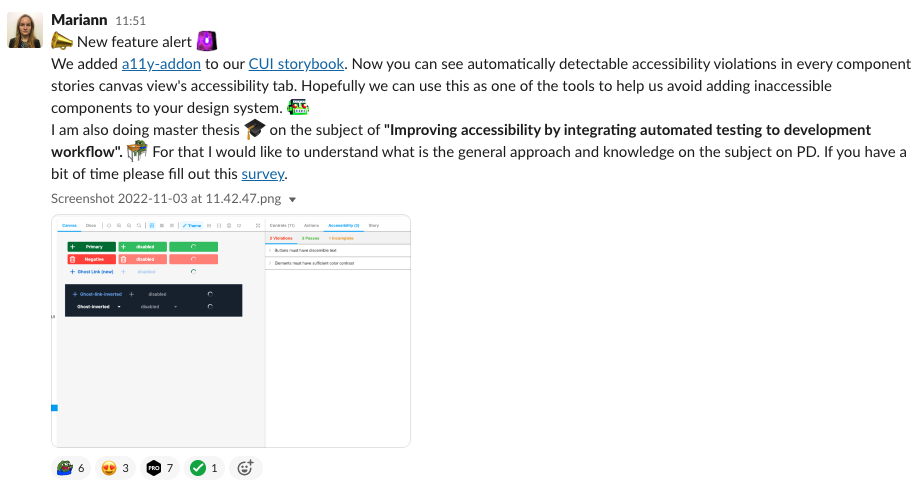
\includegraphics[width=\textwidth]{img/survey.png}
	\caption{Message in company Slack announcing adding accessibility tool and inviting people to reply to the survey.}
	\label{fig:slack-message}
\end{figure}

In total 20 people replied to the survey - 6 designers and 14 developers, including one engineering manager. This does not give a full overview of the company, but it should give a good insight into what general opinions regarding accessibility might be. Likely, developers and designers that are more involved with our component library and/or interested in accessibility were more likely to respond.

The results show that 10\% of people who responded think their knowledge of accessibility is very good, while most think that their knowledge level is average. 35\% of responders know where to find resources about accessibility standards, 15\% don't know and 50\% know, but think they need more. They don't see that accessibility as a high priority in the company currently, but at the same time, 40\% of the people who responded think that following accessibility standards should be prioritized. There were several comments in the free text sections expressing saying they appreciate this subject being opened.

\subsection{Adding automated accessibility tests to component library}
The next step was adding some automated tests to our component library development workflow and observing their usefulness. The aim was to find something that we can integrate into our development workflow without the need to learn a new tool or add unnecessary complexity.

We use Storybook for our UI development. It is an open-source software for UI development tool that allows you to work on one component at a time \citep{storybook}. It allows us to render isolated UI components without integrating them into the final product right away. Our developers use it to test out the components they are developing locally. We also have a version of Storybook available for anyone in the company to see with all the components. If this is the first place where elements will be rendered it seems logical to try to find a way to start testing them there.

To show a component you need to write a story - this means use it the way you would use it in the real world, and it will be rendered in a browser inside Storybook UI. It also has a sidebar for navigating between different examples, and controls for additional tools and documentation. This means using a browser extension for accessibility tests would also test the UI around the actual example.

\begin{figure}[h]
	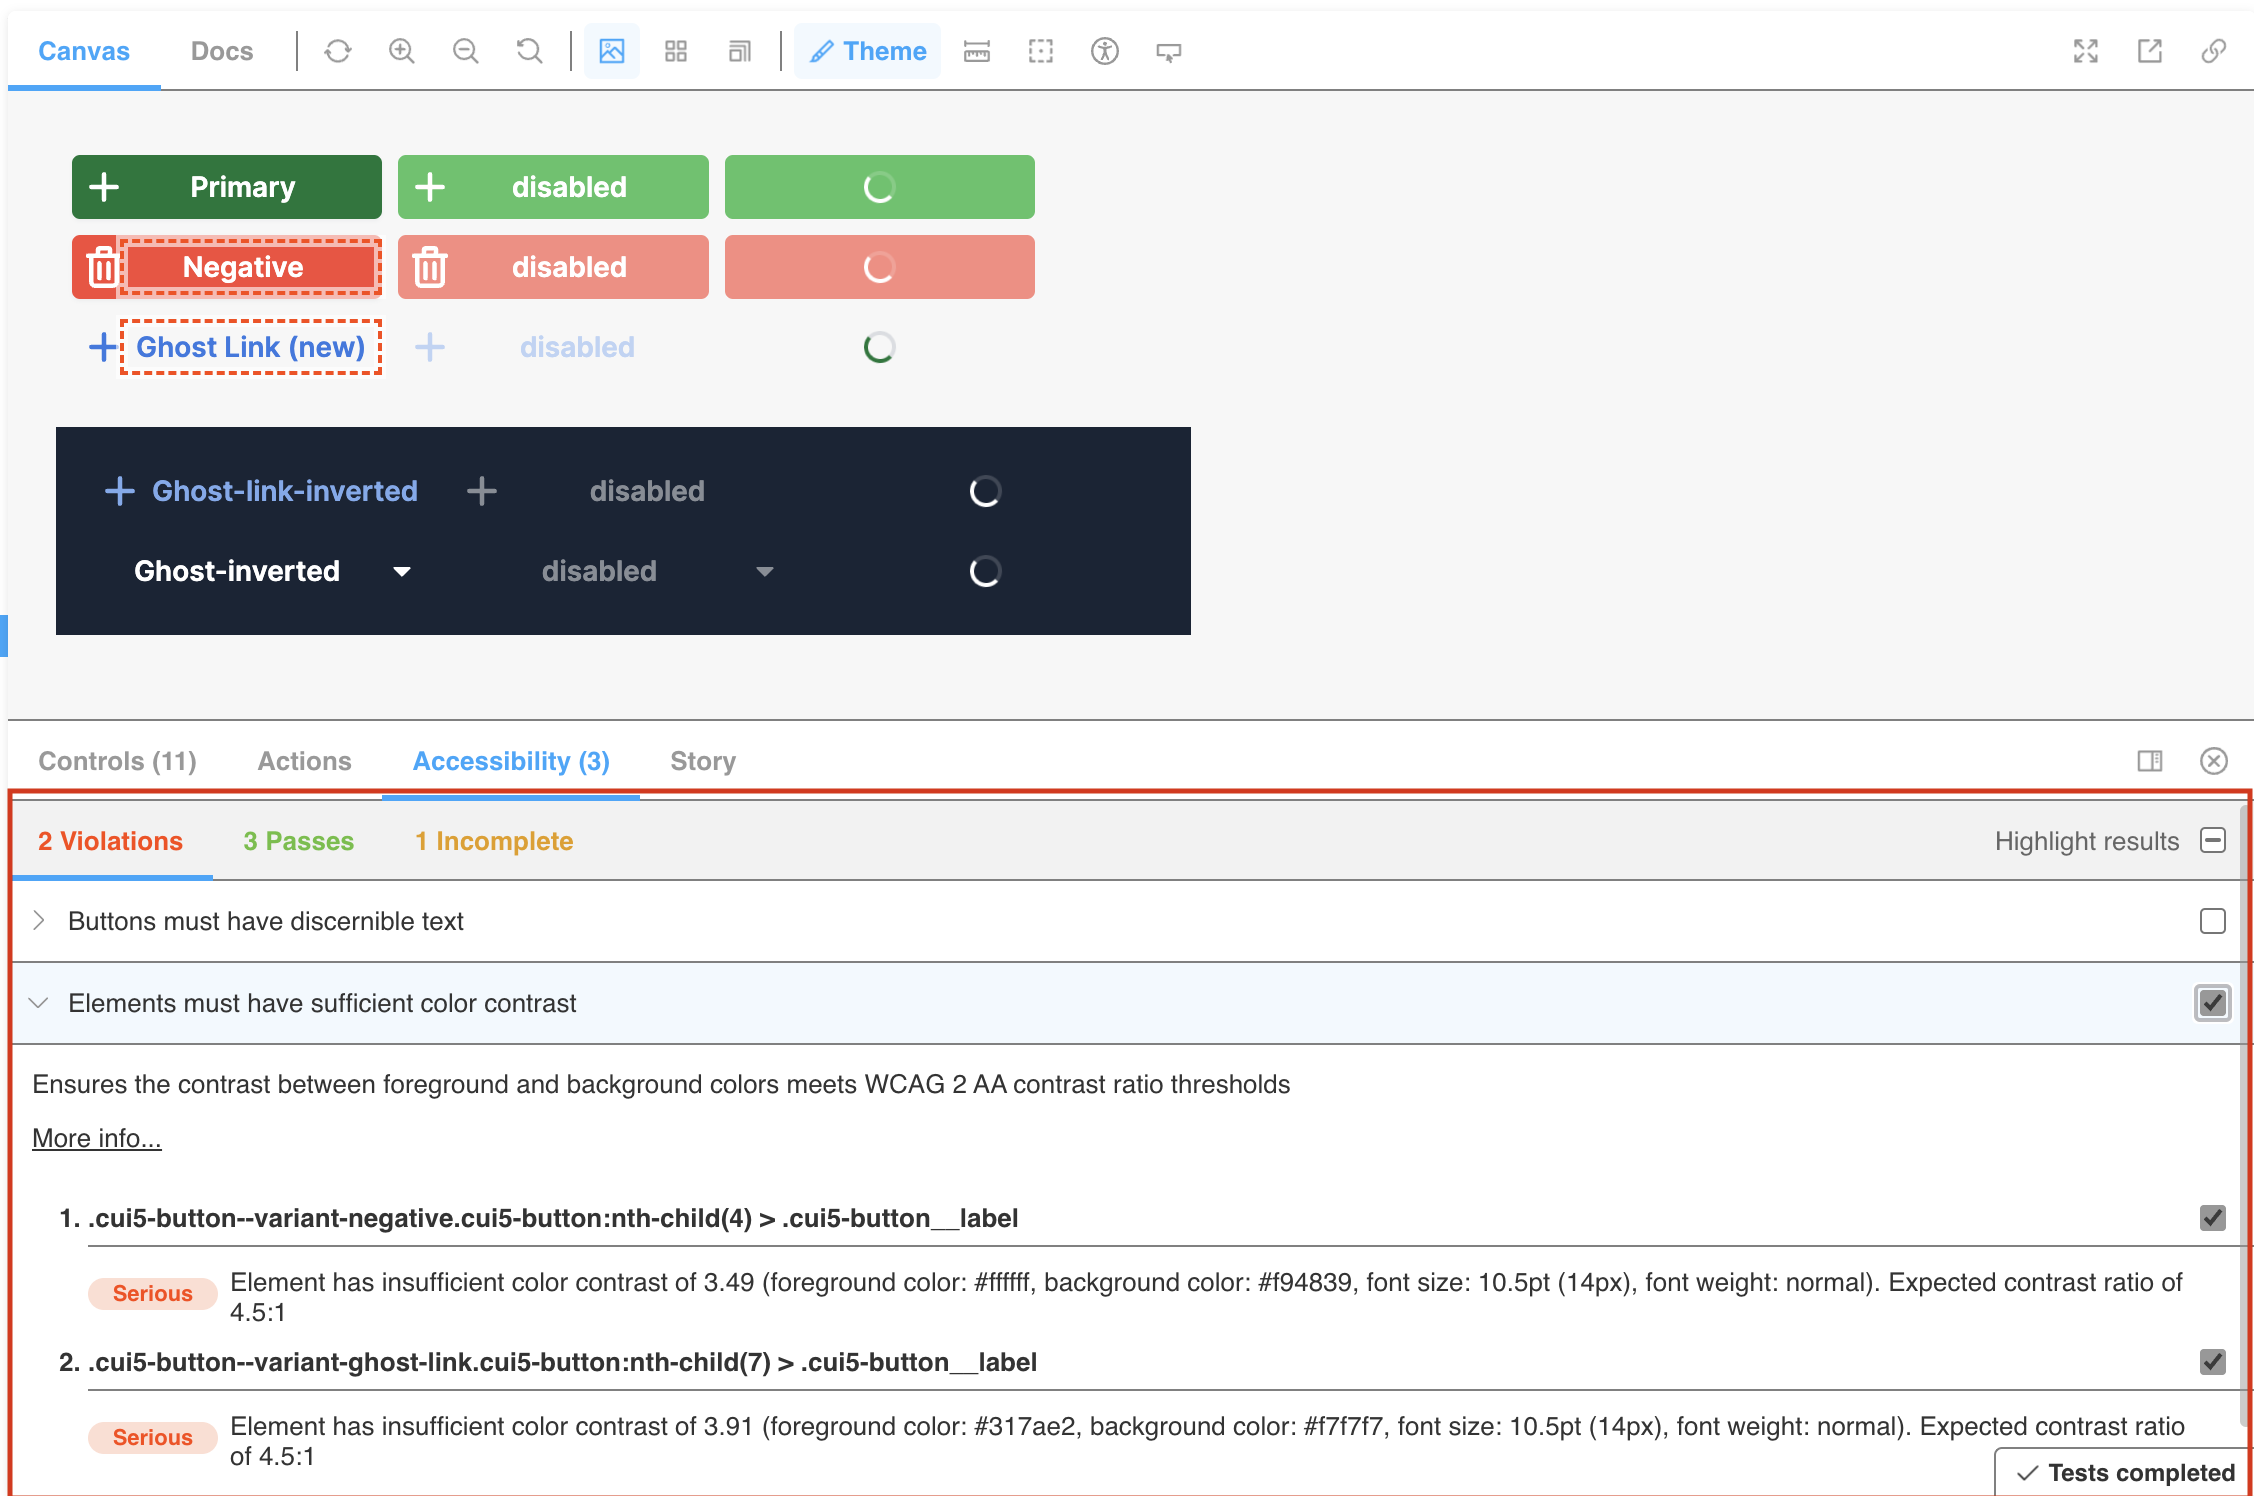
\includegraphics[width=\textwidth]{img/addon-a11y.png}
	\caption{Accessibility add-on for Storybook (addon-a11y)}
	\label{fig:addon-a11y}
\end{figure}

Storybook has a wide ecosystem of add-ons and one of them is addon-a11y (see figure \ref{fig:addon-a11y} ). It uses Deque's axe-core to audit the HTML rendered for an isolated component \citep{addon-a11y}. Axe-core is an accessibility testing engine for websites and other HTML-based user interfaces. It includes WCAG 2.0 and 2.1 on levels A and AA and promises to catch 57\% of WCAG issues on average. \citep{Deque2023} This should be taken with a grain of salt because we are intending to test isolated elements and not the whole webpage and other studies comparing accessibility testing tools' effectiveness have found the coverage to be lower  \todo{needs citation}.

This seemed like the best solution in our situation so addon-a11y was added to our component library’s storybook. The tool is visible in the sidebar of every example. It shows all the checks that it has passed, all the violations that were found and any issues that could not be checked and might need manual testing. Every rule listed there also has reference to the HTML node that had the violation, explanation and links to the Deque webpage with examples. This should be very useful in understanding and fixing these issues.

It does not generate a report of all the issues found across the whole library for this another tool was used that will go through all the examples and generate a summary of all the violations found.

The rules format that axe-core uses is developed by Deque Systems and is an adoption of the ACT rules format developed by WAI \citep{Fiers2017}. They have a set WCAG that can be evaluated in a fully automated way. They are divided by WCAG standards version (2.0, 2.1, 2.2) and Level (A \& AA, AAA) and they also have some rules for best practices in the industry that improve the user experience but might not conform to WCAG success criterion \citep{Fiers2023}.

\textbf{Data gathered from automated testing report:}
\begin{itemize}
	\item How many occurrences in the accessibility violations report? This will show how many violations were detected from all the examples. Might contain the same issue multiple times.
	\item How many unique issues will only count different violations for each component?
	\item How many passed checks – this together with violations will show how many things were tested for each component – Most components have more than one story – the list will contain all different passed checks listed
	\item How many valid checks – are the passed checks relevant to the component – only count the ones that are related to the component that the example is about.
\end{itemize}

\subsection{Manual accessibility audit}

The second part is conducting a manual accessibility audit in the same library and comparing the results with the automatically generated test report results to determine what are its strengths and weaknesses and if testing isolated components pose any limitations.
\subsubsection{Methodology for manual audit}
We used Storybook to look at an isolated preview of how each component would be rendered.
 The accessibility add-on had already been installed, and we looked at the violations reported there too. We worked in a team of 4 people - 3 designers and 1 developer. We created a task for each component - 53 tasks in total.

We checked violations in the accessibility add-on panel (see figure \todo{add figure}), tried using only a keyboard to navigate, and tried using a screen reader to navigate. Each component had 1 or more examples. As many as was relevant to get the whole picture where looked at.

At the beginning of the audit, we tested an add-on in Storybook for mocking a screen reader (\todo{Reference for this add-on and maybe an article about the difficulty of using a screen reader}). It had the option to show the output a normal screen reader would play as audio as text. Initially, it seemed like a convenient solution with rather reliable results, but further investigation revealed that the output was very different from what an actual screen reader. For the rest on the audit, we used Voice over - the MacBook built-in screen reader because it was available to us. There was an initial learning curve, but after that, it went quite smoothly. All the components that had already been tested with the faulty add-on were looked over again using VoiceOver.

The audit results were documented in a table. We approached the problems from the user's perspective and looked at what issues different types of users might encounter. We separated them into 3 sections:
\begin{enumerate}
	\item Mouse user issues
	\item Keyboard user issues
	\item Screen reader user issues
\end{enumerate}

We see this separation as a good way to prioritize fixing the issues in the future. The mouse user is the user we are considering in all of our development currently. The issues they would encounter should be the most critical. This category includes a lot of visual, color contrast and image text issues.

The second type of user would encounter all the issues from the first category plus everything that is unreachable to them by using a keyboard. We looked at what functionality is or should be working when you use a mouse and tried to do the same things by only using a keyboard.

The third user was imitated by using a screen reader. The prerequisite for this was keyboard usability - if it was not possible to navigate using a keyboard then most likely it would not be very usable by a screen reader.

In real life, these users might not be so clearly separated and many issues would affect all types of users, but as the intention was to come out of the audit with an actionable list we needed to prioritize the issues while we found them in order of severity and current customer impact. These categories also mostly depend on each other, so it would make sense in most cases to start by solving mouse user issues, then keyboard user issues and then screen reader user issues.

\end{document}